\section{Overview of \name}
\label{sec:overview}

To optimize inter-DC bulk-data multicast while avoiding
interference with latency-sensitive traffic, we present \name,
a near-optimal inter-DC multicast overlay network.
Unlike previous designs which always, to some extent, keep
some local control capability at individual servers,
\name takes an explicit stance of {\em fully centralizing} the
control of an inter-DC multicast overlay network.
Before presenting \name in more details,
we first highlight the intuitions behind this design
choice and the key challenge to make it practical.


%\name is built on a couple of design choices, which
%trade marginal costs for substantial performance benefits.
%Before describing the details of \name's design, we first
%highlight the design choices and the intuition behind
%their cost-benefit tradeoffs
%(summarized in Table~\ref{tab:design-choices}).



%The insights obtained from \company's operational experience has inspired the design of \name, a near-optimal inter-DC multicast overlay network. This section starts with \name key design choices, highlights the design philosophy behind our choices, and provide an overview of the \name system, which builds on these design choices.

%\subsection{Why a fully centralized design}

\mypara{Conventional wisdom}
The limitations of many prior approaches, including \company's
system, as highlighted in \Section\ref{subsec:motivation:baseline},
stem from the suboptimal adaptation made locally
at individual servers
based on a limited visibility of multicast states at
other servers.
These limitations remain, though to a lesser extent, in hybrid
control schemes (e.g.,~\cite{yin2009design}) where local
adaptation happens in real-time while a centralized logic
operates on more coarse timescales.
Despite this lacking of global view and coordination, the
conventional wisdom has
been that local adaptation is needed to achieve
scalability and responsiveness, and the cost of suboptimal
performance is thus deemed necessary.

\begin{figure}[t]
  \centering
  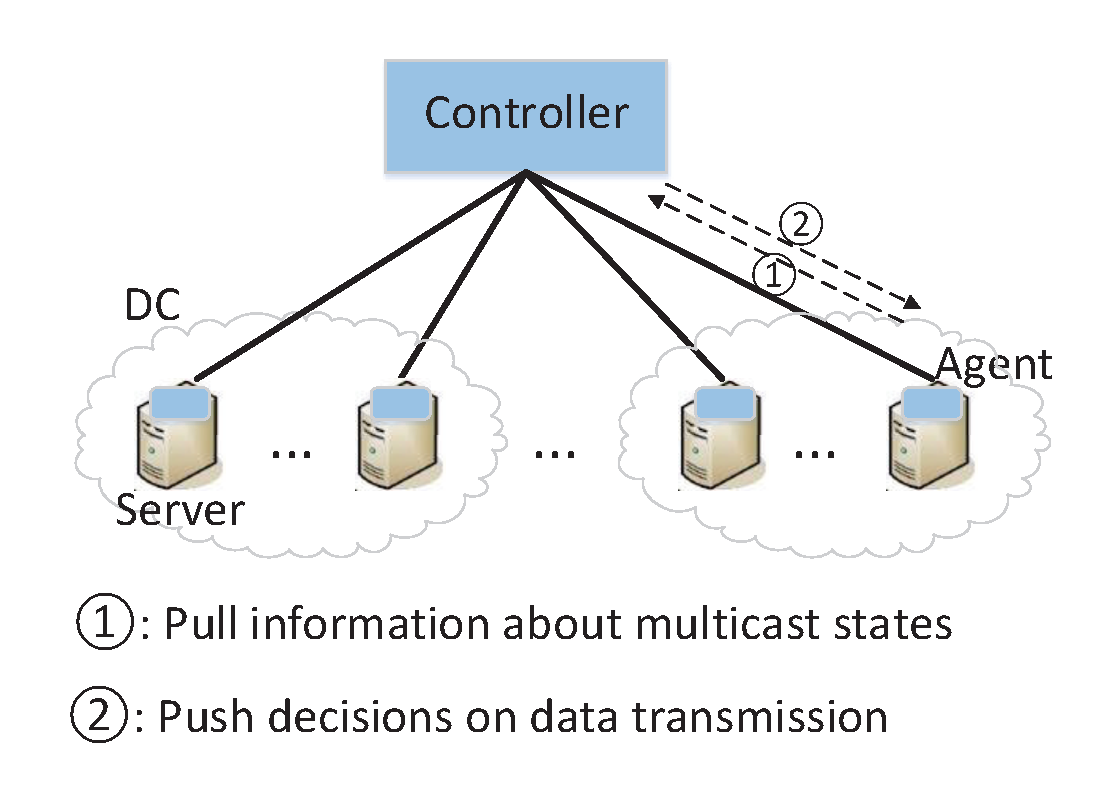
\includegraphics[width=2in]{images/framework.eps}
  \caption{The centralized design of \name.}
  \label{fig:framework}
\vspace{-0.4cm}
\end{figure}

\mypara{Centralized design}
However, we believe that such arguement does not apply in our
setting of bulk-data inter-DC multicast; instead, we argue for
a fully centralized design and demonstrate the cost of
suboptimal performance is not necessary after all.
As illustrated in Figure~\ref{fig:framework}, \name uses a centralized controller to update decisions,
including schedule of data transfers, and path selection and
bandwidth allocation of each transfer, on timescales of
several seconds.
At a high level, \name controller periodically pulls information
from all servers to maintain a most up-to-date global view of
multicast states, updates the decisions, and pushes them
to agents running locally on servers.
That said, under failure scenarios where the controller is
not available, \name will reverse to a default decentralized
overlay protocol to ensure graceful degradation on performance.

\mypara{Design philosophy}
Our intuition in favor of a centralized design is four-fold:
\begin{packedenumerate}
\item {\em Larger data sizes:}
Data sizes of bulk-data multicast are much larger
than those of overlay networks (e.g., live streaming).
This means that data transfers happen on long timescales,
potentially longer than changes in network conditions or
new job arrivals.
Therefore, being highly responsive to network congestions
is secondary.
Instead, we can tolerate a small delay of several seconds for
querying a centralized controller,
in exchange for closer-to-optimal scheduling decisions.
\item {\em Larger decision space:}
Given the sheer number of inter-DC overlay paths,
which grows exponentially with more servers that can
serve as overlay nodes,
it is hard for individual servers to explore possible overlay
paths based only on its local measurements.
Instead, overlay routing must be driven by a global
view of across all servers in order to
balance the availability across different data blocks, which
turned out to be critical to achieve near-optimal performance.
\item {\em Need for more strict traffic control:}
As observed in \Section\ref{subsec:motivation:baseline}, it is vital that inter-DC
bulk-data multicast avoids hotspots and excessive use of
bandwidth that could interference with latency sensitive traffic.
While it is difficult to enforce a limit on outgoing traffic
without any coordination across overlay servers, it is practical
to determine the bandwidth allocation and periodically update it
to all servers in a centralized fashion.
\item {\em Engineeringly simpler:}
In some sense, the resulting centralized system is conceptually
simpler and amenable to a simple implementation.
For instance, the control logic running locally in each server
is only triggered on arrivals of new data units or control messages,
and thus can be stateless and lightweight.

\end{packedenumerate}

\mypara{Fast and optimal decision-making is the key}
In essence, \name trades updating decisions on coarse timescales
for the potential of making optimal decisions in a centralized
fashion.
Therefore, the key to striking a favorable is a
{\em near-optimal and efficient overlay routing
algorithm} that can be updated on near-realtime timescales of
several seconds.
At a first glance, this is indeed intractable:
the centralized overlay routing algorithm must pick the next hops
from 10,000s servers for 10,000s objects, a scale that could
even explode exponentially, as we consider all possible
overlay paths that go through these servers, and chop each data
object into many fine-grained blocks to enable fine-grained
multipath overlay routing.
It is unclear how this problem can be solved even with
limited approximation, which was why for many years, \company have
relied on decentralized protocols for bulk-data multicast.
The next section  will present how \name addresses this
challenge.

%The key technical challenge here is how to make optimal overlay scheduling and routing decisions at the scale tens of thousands of objects and tens of thousands of servers in near real time. To achieve desirable performance in a multicast overlay network, fully exploiting all the available overlay paths is essential, but it is untenable to go through all the potential servers and exponentially more paths by traditional approaches.

%\begin{itemize}
%
%\item Idea \#1: Fully centralized control
%
%\item Idea \#2: Dynamic bandwidth separation: separating background bulk data transfer from latency-sensitive traffic
%
%\item These ideas introduces performance costs (not real time, potentially low link utilization) are outweighed by benefits (not real time, potentially low link utilization)
%
%\item Design philosophy: the costs are outweighed by the benefits. (1) bulk data transfer can tolerate updates at coarse timescales. (2) the aggregation of latency-sensitive data is stable on timescales of several seconds. (3) the resulting system is amenable to simpler implementation.
%
%\item Key technical challenge: how to make optimal overlay scheduling and routing decisions at the scale tens of thousands of objects and tens of thousands of servers in near real time.
%
%\end{itemize}



